\chapter{Características de la interfaz}

\section{Introducción a la interfaz}

SimAS 3.0 presenta una interfaz moderna e intuitiva desarrollada con JavaFX \cite{javafx} que facilita el aprendizaje y uso de la aplicación. La interfaz está diseñada para ser clara, accesible y funcional, permitiendo a los usuarios concentrarse en los conceptos de análisis sintáctico sin distracciones innecesarias.

La aplicación utiliza un sistema de pestañas que permite trabajar con múltiples gramáticas y simulaciones simultáneamente, mejorando significativamente la productividad del usuario.

\section{Pantalla de bienvenida}

Al iniciar SimAS 3.0, la primera pantalla que aparece es la pantalla de bienvenida, que incluye:

\begin{itemize}
    \item \textbf{Logo de la aplicación}: identificación visual clara de SimAS 3.0.
    \item \textbf{Información de versión}: muestra la versión actual de la aplicación.
    \item \textbf{Credenciales del desarrollador}: información sobre el autor y director del proyecto.
    \item \textbf{Indicador de progreso}: muestra el estado de carga de los componentes de la aplicación.
\end{itemize}

Esta pantalla permanece visible durante unos segundos mientras la aplicación inicializa todos sus componentes y recursos necesarios.

\section{Menú principal}

Una vez completada la carga, la aplicación muestra el menú principal, que constituye el centro de navegación de SimAS 3.0.

\subsection{Elementos del menú principal}

El menú principal, mostrado en la figura \ref{fig:menu_principal}, incluye los siguientes elementos:

\begin{itemize}
    \item \textbf{Título de la aplicación}: \string"SimAS 3.0\string" en la parte superior.
    \item \textbf{Subtítulo}: \string"Simulador de Análisis Sintáctico\string" que describe la funcionalidad.
    \item \textbf{Botones de navegación}: acceso a las principales funcionalidades.
    \item \textbf{Selector de idioma}: en la esquina superior derecha.
    \item \textbf{Información del desarrollador}: en la parte inferior.
\end{itemize}

\needspace{8cm}
\begin{figure}[H]
    \centering
    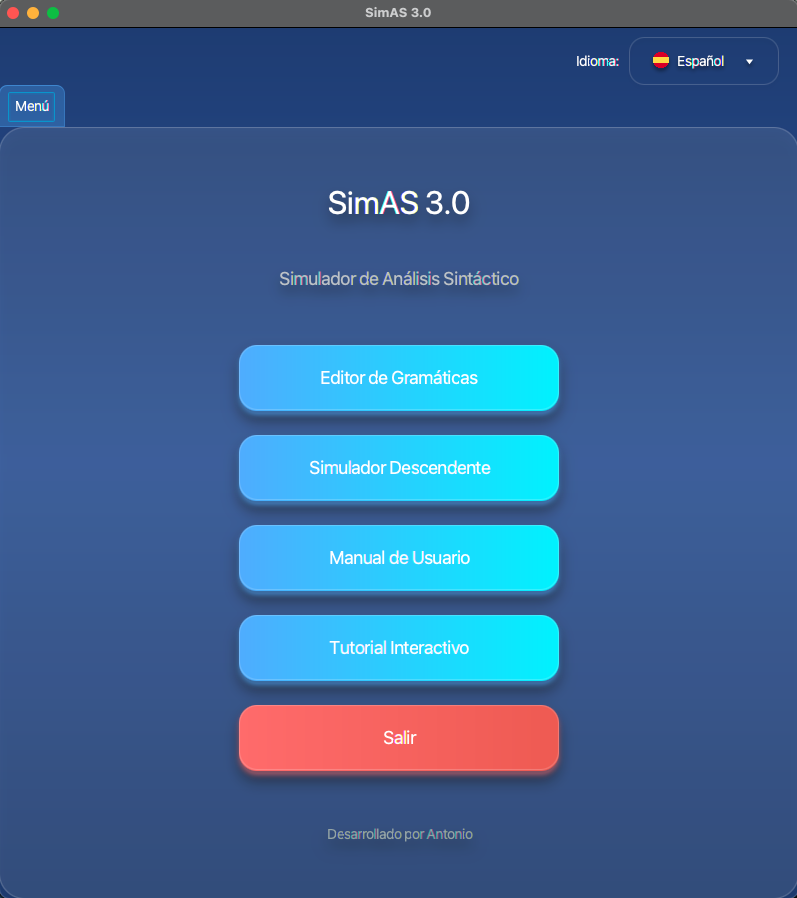
\includegraphics[width=0.9\textwidth]{figuras/menu.png}
    \caption{Menú principal de SimAS 3.0}
    \label{fig:menu_principal}
\end{figure}

\subsection{Botones principales}

Los botones del menú principal proporcionan acceso a las funcionalidades principales:

\begin{itemize}
    \item \textbf{Editor de gramáticas}: abre el editor para crear y gestionar gramáticas.
    \item \textbf{Simulador descendente}: accede al simulador de análisis sintáctico.
    \item \textbf{Manual de usuario}: abre este manual de usuario.
    \item \textbf{Tutorial interactivo}: proporciona una guía paso a paso.
    \item \textbf{Salir}: cierra la aplicación.
\end{itemize}

\section{Sistema de pestañas}

SimAS 3.0 implementa un sistema de pestañas avanzado que permite trabajar con múltiples elementos simultáneamente.

\subsection{Características del sistema de pestañas}

\begin{itemize}
    \item \textbf{Pestaña principal}: siempre visible, contiene el menú principal.
    \item \textbf{Pestañas dinámicas}: se crean automáticamente al abrir editores o simuladores.
    \item \textbf{Numeración automática}: las pestañas se numeran secuencialmente para facilitar la identificación.
    \item \textbf{Cierre individual}: cada pestaña puede cerrarse independientemente.
    \item \textbf{Reordenamiento}: las pestañas pueden arrastrarse para cambiar su orden.
\end{itemize}

\subsection{Gestión de pestañas}

\begin{itemize}
    \item \textbf{Botón \string"Cerrar todas las pestañas\string"}: cierra todas las pestañas excepto la principal.
    \item \textbf{Menú contextual}: clic derecho en una pestaña para opciones adicionales.
    \item \textbf{Separación de pestañas}: arrastrar una pestaña fuera del área principal crea una nueva ventana.
    \item \textbf{Reunión de ventanas}: arrastrar pestañas entre ventanas las consolida.
    \item \textbf{Grupos de pestañas}: las pestañas relacionadas (editor y simulador) se agrupan automáticamente.
    \item \textbf{Movimiento de grupos}: arrastrar una pestaña de un grupo mueve todo el grupo a una nueva ventana.
    \item \textbf{Numeración de grupos}: cada grupo de pestañas recibe un número único para identificación.
\end{itemize}

\section{Selector de idioma}

SimAS 3.0 soporta múltiples idiomas, permitiendo a los usuarios trabajar en su idioma preferido.

\subsection{Idiomas disponibles}

La aplicación incluye soporte para los siguientes idiomas:

\begin{itemize}
    \item \textbf{Español}: idioma por defecto.
    \item \textbf{English}: inglés.
    \item \textbf{Français}: francés.
    \item \textbf{Português}: portugués.
    \item \textbf{Deutsch}: alemán.
    \item \textbf{Japanese}: japonés.
\end{itemize}

\subsection{Cambio de idioma}

Para cambiar el idioma de la interfaz:

\begin{enumerate}
    \item Localice el selector de idioma en la esquina superior derecha de la ventana principal de la aplicación.
    \item Haga clic en el menú desplegable.
    \item Seleccione el idioma deseado de la lista.
    \item La interfaz se actualizará inmediatamente al nuevo idioma.
    \item El cambio se aplicará a todas las pestañas y ventanas abiertas.
    \item El idioma seleccionado se mantiene durante toda la sesión de trabajo.
\end{enumerate}

\needspace{8cm}
\begin{figure}[H]
    \centering
    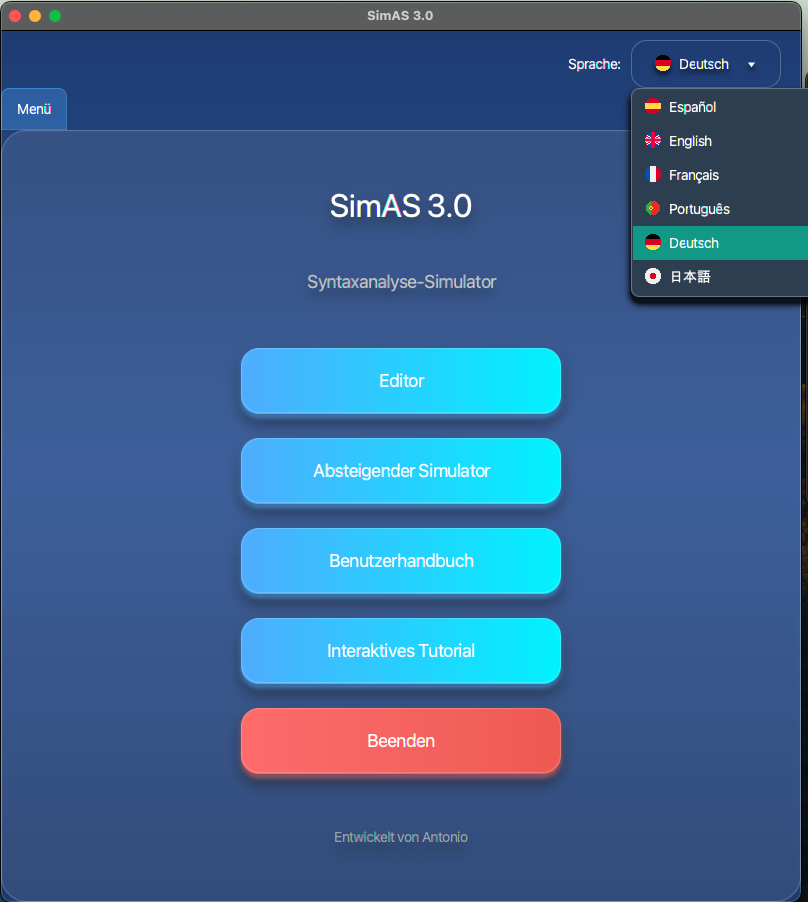
\includegraphics[width=0.9\textwidth]{figuras/menu_idiomas.png}
    \caption{Selector de idiomas con menú desplegable}
    \label{fig:menu_idiomas}
\end{figure}

El selector de idiomas, ilustrado en la figura \ref{fig:menu_idiomas}, muestra todos los idiomas disponibles en un menú desplegable fácil de usar.

\section{Atajos de teclado}

SimAS 3.0 incluye atajos de teclado para facilitar el acceso rápido a las funciones principales.

\subsection{Atajos disponibles}

SimAS 3.0 incluye los siguientes atajos de teclado:

\begin{itemize}
    \item \textbf{Ctrl+N}: abre el editor de gramáticas.
    \item \textbf{Ctrl+S}: abre el simulador descendente.
    \item \textbf{Ctrl+H}: abre el manual de usuario.
    \item \textbf{Ctrl+W}: cierra la pestaña actual.
    \item \textbf{Ctrl+Shift+W}: cierra todas las pestañas. 
    \item \textbf{Ctrl+Tab}: navega a la siguiente pestaña.
    \item \textbf{Ctrl+Shift+Tab}: navega a la pestaña anterior.
    \item \textbf{Ctrl+T}: crea una nueva pestaña del editor.
    \item \textbf{Ctrl+Shift+T}: crea una nueva ventana.
    \item \textbf{Ctrl+1-9}: navega directamente a la pestaña numerada.
\end{itemize}

\subsection{Uso de atajos}

Los atajos de teclado funcionan desde cualquier pestaña activa y proporcionan acceso rápido a las funcionalidades más utilizadas, mejorando la eficiencia del usuario.

\section{Elementos visuales}

La interfaz de SimAS 3.0 utiliza elementos visuales consistentes para mejorar la experiencia del usuario.

\subsection{Iconos y gráficos}

\begin{itemize}
    \item \textbf{Iconos descriptivos}: cada botón principal incluye un icono que representa su función.
    \item \textbf{Banderas de países}: el selector de idioma muestra banderas para identificación visual.
    \item \textbf{Indicadores de estado}: elementos visuales que muestran el estado de las operaciones.
    \item \textbf{Colores consistentes}: paleta de colores coherente en toda la aplicación.
\end{itemize}

\subsection{Tipografía y espaciado}

\begin{itemize}
    \item \textbf{Fuentes legibles}: tipografía clara y fácil de leer.
    \item \textbf{Espaciado apropiado}: elementos bien distribuidos para evitar saturación visual.
    \item \textbf{Jerarquía visual}: diferentes tamaños de fuente para establecer importancia.
    \item \textbf{Contraste adecuado}: colores que facilitan la lectura.
\end{itemize}

\section{Responsividad de la interfaz}

La interfaz de SimAS 3.0 está diseñada para adaptarse a diferentes tamaños de pantalla y resoluciones.

\subsection{Adaptación a la pantalla}

\begin{itemize}
    \item \textbf{Tamaño mínimo}: la ventana puede redimensionarse hasta 600x700 píxeles.
    \item \textbf{Tamaño por defecto}: 800x900 píxeles para una experiencia óptima.
    \item \textbf{Escalado automático}: los elementos se adaptan al tamaño de la ventana.
    \item \textbf{Barras de desplazamiento}: aparecen automáticamente cuando es necesario.
\end{itemize}

\subsection{Optimización para diferentes resoluciones}

La aplicación se optimiza automáticamente para:

\begin{itemize}
    \item \textbf{Resoluciones estándar}: 1024x768, 1366x768, 1920x1080.
    \item \textbf{Pantallas de alta densidad}: soporte para pantallas Retina y similares.
    \item \textbf{Orientaciones}: funciona correctamente en orientación horizontal.
    \item \textbf{Proporciones}: se adapta a diferentes relaciones de aspecto.
\end{itemize}

\section{Accesibilidad}

SimAS 3.0 incluye características de accesibilidad para facilitar su uso por parte de todos los usuarios.

\subsection{Características de accesibilidad}

\begin{itemize}
    \item \textbf{Atajos de teclado}: alternativa al uso del ratón.
    \item \textbf{Contraste visual}: colores que facilitan la distinción de elementos.
    \item \textbf{Tamaño de fuente}: texto legible en diferentes tamaños de pantalla.
    \item \textbf{Navegación por teclado}: todos los elementos son accesibles mediante teclado.
\end{itemize}

\subsection{Compatibilidad con tecnologías asistivas}

La aplicación es compatible con:

\begin{itemize}
    \item \textbf{Amplificadores de pantalla}: elementos visuales claros y contrastados.
    \item \textbf{Dispositivos de entrada alternativos}: soporte para diferentes tipos de entrada (ratón, teclado, trackpad).
    \item \textbf{Software de control por voz}: compatible con sistemas de control por voz del sistema operativo.
    \item \textbf{Dispositivos de entrada adaptativos}: soporte para dispositivos especializados de accesibilidad.
\end{itemize}

\section{Personalización de la interfaz}

Aunque SimAS 3.0 mantiene una apariencia consistente, los usuarios pueden personalizar algunos aspectos de la experiencia.

\subsection{Opciones de personalización}

\begin{itemize}
    \item \textbf{Idioma}: selección del idioma de la interfaz.
    \item \textbf{Tamaño de ventana}: redimensionamiento según preferencias.
    \item \textbf{Organización de pestañas}: reordenamiento y agrupación.
    \item \textbf{Atajos de teclado}: uso opcional de atajos para funciones rápidas.
\end{itemize}

\subsection{Limitaciones de personalización}

Por motivos de consistencia y funcionalidad, algunos elementos no son personalizables:

\begin{itemize}
    \item \textbf{Colores de la interfaz}: paleta fija para mantener coherencia visual.
    \item \textbf{Tipografía}: fuente estándar para garantizar legibilidad.
    \item \textbf{Disposición de elementos}: estructura fija para optimizar el flujo de trabajo.
    \item \textbf{Iconos}: conjunto estándar para facilitar el reconocimiento.
\end{itemize}

\section{Integración entre componentes}

La interfaz de SimAS 3.0 está diseñada para facilitar la integración entre diferentes componentes de la aplicación.

\subsection{Flujo de trabajo integrado}

\begin{itemize}
    \item \textbf{Editor a simulador}: transición directa desde el editor al simulador.
    \item \textbf{Sincronización de datos}: las gramáticas se comparten automáticamente entre componentes.
    \item \textbf{Estado consistente}: cambios en un componente se reflejan en otros.
    \item \textbf{Navegación fluida}: transiciones suaves entre diferentes funcionalidades.
\end{itemize}

\subsection{Comunicación entre ventanas}

\begin{itemize}
    \item \textbf{Ventanas secundarias}: creación de ventanas adicionales para trabajo paralelo.
    \item \textbf{Sincronización de idioma}: cambios de idioma se aplican a todas las ventanas.
    \item \textbf{Gestión de estado}: estado compartido entre ventanas relacionadas.
    \item \textbf{Cierre coordinado}: cierre apropiado de ventanas dependientes.
\end{itemize}

\section{Solución de problemas de interfaz}

Si experimenta problemas con la interfaz de SimAS 3.0, considere las siguientes soluciones:

\subsection{Problemas comunes}

\begin{itemize}
    \item \textbf{Interfaz no se muestra correctamente}: verifique la resolución de pantalla y actualice los controladores gráficos.
    \item \textbf{Elementos superpuestos}: redimensione la ventana o cambie la resolución de pantalla.
    \item \textbf{Texto borroso}: ajuste la configuración de escalado de Windows/macOS.
    \item \textbf{Atajos de teclado no funcionan}: asegúrese de que la ventana esté activa y enfocada.
\end{itemize}

\subsection{Optimización del rendimiento}

Para obtener el mejor rendimiento de la interfaz:

\begin{itemize}
    \item \textbf{Cierre pestañas innecesarias}: mantenga solo las pestañas que esté utilizando.
    \item \textbf{Resolución apropiada}: use una resolución de pantalla compatible.
    \item \textbf{Memoria disponible}: asegúrese de tener suficiente memoria RAM libre.
    \item \textbf{Controladores actualizados}: mantenga actualizados los controladores gráficos.
\end{itemize}

\section{Ventanas secundarias}

SimAS 3.0 permite crear ventanas secundarias para trabajar con múltiples proyectos simultáneamente, mejorando significativamente la productividad del usuario.

\subsection{Creación de ventanas secundarias}

Las ventanas secundarias se pueden crear de las siguientes maneras:

\begin{itemize}
    \item \textbf{Arrastrando pestañas}: arrastrar una pestaña fuera del área principal crea automáticamente una nueva ventana.
    \item \textbf{Menú contextual}: clic derecho en una pestaña y seleccionar \string"Nueva ventana\string".
\end{itemize}

\subsection{Características de las ventanas secundarias}

Cada ventana secundaria mantiene las siguientes características:

\begin{itemize}
    \item \textbf{Independencia}: cada ventana funciona de manera independiente.    
    \item \textbf{Sincronización de idioma}: cambios de idioma se aplican a todas las ventanas.
    \item \textbf{Gestión de pestañas}: cada ventana tiene su propio sistema de pestañas.
    \item \textbf{Estado persistente}: el estado de cada ventana se mantiene durante la sesión.
    \item \textbf{Comunicación entre ventanas}: las ventanas pueden compartir datos cuando es necesario.
\end{itemize}

\subsection{Gestión de múltiples ventanas}

Para gestionar eficientemente múltiples ventanas:

\begin{itemize}
    \item \textbf{Organización}: cada ventana puede contener un proyecto diferente.
    \item \textbf{Intercambio de datos}: arrastrar pestañas entre ventanas para reorganizar el trabajo.
    \item \textbf{Cierre coordinado}: cerrar una ventana principal cierra todas las ventanas secundarias.
\end{itemize}

\section{Barra de estado y notificaciones}

SimAS 3.0 incluye una barra de estado que proporciona información importante sobre el estado de la aplicación y las operaciones en curso.

\subsection{Elementos de la barra de estado}

La barra de estado incluye:

\begin{itemize}
    \item \textbf{Mensajes informativos}: notificaciones sobre el estado del sistema.
    \item \textbf{Contador de pestañas}: número total de pestañas abiertas.
    \item \textbf{Indicador de idioma}: idioma actualmente seleccionado.
\end{itemize}

\subsection{Sistema de notificaciones}

El sistema de notificaciones proporciona:

\begin{itemize}
    \item \textbf{Notificaciones de éxito}: confirmación de operaciones completadas.
    \item \textbf{Advertencias}: alertas sobre posibles problemas.
    \item \textbf{Errores}: información detallada sobre errores encontrados.
    \item \textbf{Información contextual}: ayuda específica según la situación.
\end{itemize}

\section{Menús contextuales}

SimAS 3.0 implementa menús contextuales inteligentes que se adaptan al contexto actual.

\subsection{Menús contextuales de pestañas}

Al hacer clic derecho en una pestaña, se muestra un menú con opciones como:

\begin{itemize}
    \item \textbf{Cerrar pestaña}: cierra la pestaña actual.
    \item \textbf{Cerrar todas las pestañas}: cierra todas las pestañas de la ventana actual.
    \item \textbf{Abrir en nueva ventana}: abre la pestaña en una nueva ventana.
    \item \textbf{Abrir en ventana existente}: abre la pestaña en una ventana existente.
\end{itemize}


\section{Conclusión}

La interfaz de SimAS 3.0 está diseñada para proporcionar una experiencia de usuario intuitiva, eficiente y profesional. Con su sistema de pestañas avanzado, soporte multiidioma completo, atajos de teclado extensivos, características de accesibilidad robustas e integración profunda con el sistema operativo, la aplicación facilita el aprendizaje y uso de los conceptos de análisis sintáctico descendente predictivo.

La capacidad de trabajar con múltiples elementos simultáneamente, la gestión inteligente de ventanas secundarias, los menús contextuales adaptativos y la configuración avanzada hacen de SimAS 3.0 una herramienta poderosa, flexible y profesional para estudiantes, profesores e investigadores en el campo de la informática y la teoría de lenguajes formales.

La interfaz no solo cumple con los estándares de usabilidad modernos, sino que también establece nuevas referencias en el campo de las aplicaciones educativas especializadas, proporcionando una experiencia de usuario a la altura de las mejores herramientas profesionales del mercado.